\documentclass[12pt, a4paper, twoside]{article}
% font size could be 10pt (default), 11pt or 12 pt
% paper size coulde be letterpaper (default), legalpaper, executivepaper,
% a4paper, a5paper or b5paper
% side coulde be oneside (default) or twoside 
% columns coulde be onecolumn (default) or twocolumn
% graphics coulde be final (default) or draft 
%
% titlepage coulde be notitlepage (default) or titlepage which 
% makes an extra page for title 
% 
% paper alignment coulde be portrait (default) or landscape 
%
% equations coulde be 
%   default number of the equation on the rigth and equation centered 
%   leqno number on the left and equation centered 
%   fleqn number on the rigth and  equation on the left side
%

\usepackage{graphicx}
\usepackage{subcaption}

\usepackage{fullpage}

\usepackage{setspace}
\doublespacing

\title{Assignment 2\\\vspace{-2ex}{\large Parallel Architectures}}
\author{Rodrigo C. O. Rocha}
\date{\vspace{-2.5ex}{\large s1533346}}

%\linespread{0.7}
% \date{\today} date coulde be today 
% \date{25.12.00} or be a certain date
% \date{ } or there is no date 
\begin{document}
% Hint: \title{what ever}, \author{who care} and \date{when ever} could stand 
% before or after the \begin{document} command 
% BUT the \maketitle command MUST come AFTER the \begin{document} command! 

\maketitle

%\begin{abstract}
%\end{abstract}

%\tableofcontents % create a table of contens

\section{Introduction}

In this work, we implement a cache simulator to compared several cache-coherence protocol in a multi-core processor
with a single level of cache.
Section~\ref{sec:msi-snooping} we describe our implementation for the MSI snooping protocol.
Section~\ref{sec:directory-based} we describe our implementation for the directory-based protocol.
Finally, in Section~\ref{sec:mesi-snooping-2lvl} we describe our implementation for the MESI snooping protocol,
including the addition of a second-level shared cache.
For each cache-coherence protocol, we evaluate its performance in two work-load traces.

\begin{figure}
\centering
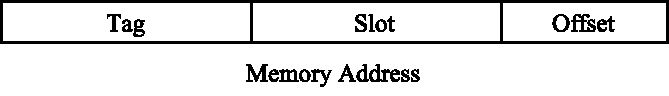
\includegraphics{figs/DirectMappedCacheAddress.pdf}
\caption{Memory address decomposed into a direct mapped cache.}
\label{fig:direct-mapping}
\end{figure}

In all cases, we consider \textit{direct mapped caches}.
In direct mapped caches, the main memory is divided into blocks of memory locations, storing multiple words per block,
and caches are organised by lines, called \textit{cache lines}. Each cache line is capable of storing exactly one memory block,
a tag that uniquely identifies the corresponding memory block, and the current state of the cache line.
Considering this organisation, the direct mapping divides each memory address into \textit{tag}, \textit{slot} and \textit{offset},
as illustrated by Figure~\ref{fig:direct-mapping}. The offset represents the word index within the memory block,
the slot represents the index of the cache line, and the tag uniquely identifies the memory address, given that we know the
corresponding slot and offset.

In this report, we consider architectures with blocks of size 4, i.e., 2 bits of offset,
and caches with 512 lines, i.e., 9 bits of slots, and the remaining 21 bits,
considering a 32 bits memory address, for the tag.

\section{MSI Snooping Protocol} \label{sec:msi-snooping}

For the MSI snooping protocol, we consider the architecture illustrated in Figure~\ref{fig:msi-arch},
where the cores are inter-connected by an unidirectional ring.

\begin{figure}[h]
\centering
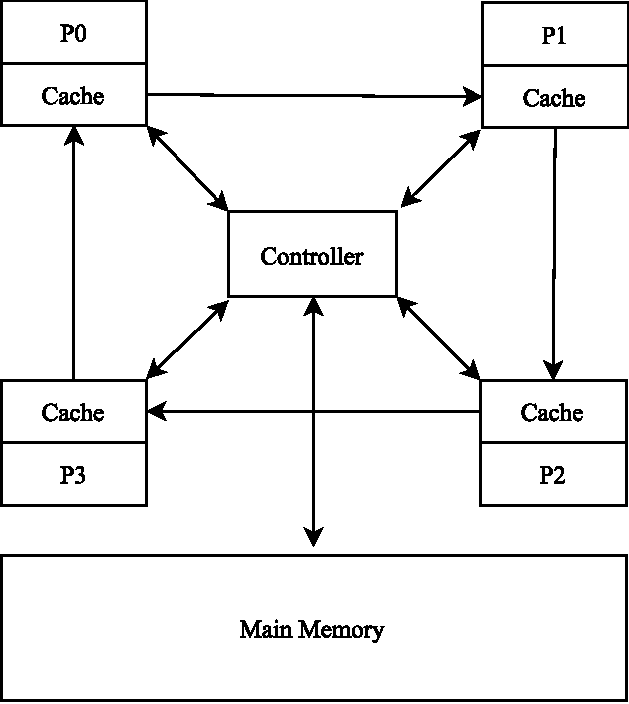
\includegraphics{figs/MSISnoopingCache.pdf}
\caption{Diagram of the architecture used with the MSI snooping protocol.}
\label{fig:msi-arch}
\end{figure}

In order to verify the correctness of the implementation, we show several small
traces executed in verbose mode.

\begin{figure}[h]
\begin{verbatim}
P1 R 10
Processor P1 reads word in address 10, with tag 0 and slot 2.
A cache miss occurred. Data transferred from main memory.
(33 cycles taken)
P1 R 10
Processor P1 reads word in address 10, with tag 0 and slot 2.
A cache hit occurred with cache line found in state Shared.
(2 cycles taken)
\end{verbatim}
\caption{(MSI Snooping Protocol) Test case: Reads with cache miss and cache hit.}
\end{figure}


\begin{figure}[h]
\begin{verbatim}
P1 R 10
Processor P1 reads word in address 10, with tag 0 and slot 2.
A cache miss occurred. Data transferred from main memory.
(33 cycles taken)
P3 R 10
Processor P3 reads word in address 10, with tag 0 and slot 2.
A cache miss occurred. Data transferred from processor P1,
found in state Shared.
(17 cycles taken)
P1 W 10
Processor P1 writes word in address 10, with tag 0 and slot 2.
Cache line found in state Shared. A total of 1 invalidations were required.
(17 cycles taken)
\end{verbatim}
\caption{(MSI Snooping Protocol) Test case: Write at P1; Local cache line in S state, Remote cache line at
P3 in S state; Expected 17 cycles.}
\end{figure}


\begin{figure}[h]
\begin{verbatim}
P1 R 10
Processor P1 reads word in address 10, with tag 0 and slot 2.
A cache miss occurred. Data transferred from main memory.
(33 cycles taken)
P2 W 10
Processor P2 writes word in address 10, with tag 0 and slot 2.
A cache miss occurred. Data transferred from processor P1,
found in state Shared. A total of 1 invalidations were required.
(18 cycles taken)
P3 R 10
Processor P3 reads word in address 10, with tag 0 and slot 2.
A cache miss occurred. Data transferred from processor P2,
found in state Modified. A protocol writeback was required by processor P2.
(18 cycles taken)
P1 W 10
Processor P1 writes word in address 10, with tag 0 and slot 2.
A cache miss occurred due to state Invalid.
Data transferred from processor P2, found in state Shared.
A total of 2 invalidations were required.
(18 cycles taken)
\end{verbatim}
\caption{(MSI Snooping Protocol) Test case: Write at P1; Local cache line in I state, Remote cache line at
P2, P3 in S state; Expected 18 cycles.}
\end{figure}


\begin{figure}[h]
\begin{verbatim}
P1 R 10
Processor P1 reads word in address 10, with tag 0 and slot 2.
A cache miss occurred. Data transferred from main memory.
(33 cycles taken)
P2 W 10
Processor P2 writes word in address 10, with tag 0 and slot 2.
A cache miss occurred. Data transferred from processor P1,
found in state Shared. A total of 1 invalidations were required.
(18 cycles taken)
P1 R 10
Processor P1 reads word in address 10, with tag 0 and slot 2.
A cache miss occurred due to state Invalid.
Data transferred from processor P2, found in state Modified.
A protocol writeback was required by processor P2.
(16 cycles taken)
\end{verbatim}
\caption{(MSI Snooping Protocol) Test case: Read at P1; Local cache line in I state, Remote cache line at
P2 in M state; Expected 19 cycles.}
\end{figure}

\begin{figure}[h]
\centering
\begin{subfigure}{0.48\textwidth}
\begin{verbatim}
Trace 1
Total Reads: 163840
Total Writes: 32768
Total Requests: 196608
Hit Rate: 0.912679036458
Direct Write: 24440
Invalidations: 51
Invalidation Sent: 8328
Private Accesses: 179440
Remote Accesses: 8427
Off-chip Accesses: 8741
Protocol Writeback: 51
Replacement Writeback: 6357
Total Cycle Count: 790691
Mean Cycle Per Req.: 4.02166239421
\end{verbatim}
\end{subfigure}
\begin{subfigure}{0.48\textwidth}
\begin{verbatim}
Trace 2
Total Reads: 507093
Total Writes: 76462
Total Requests: 583555
Hit Rate: 0.84227022303
Direct Write: 34942
Invalidations: 52559
Invalidation Sent: 41520
Private Accesses: 491511
Remote Accesses: 91537
Off-chip Accesses: 507
Protocol Writeback: 39537
Replacement Writeback: 0
Total Cycle Count: 2547924
Mean Cycle Per Req.: 4.36621055428
\end{verbatim}
\end{subfigure}
\caption{Statistics for the MSI protocol on Traces 1 and 2.}
\end{figure}

\section{Directory-based Protocol} \label{sec:directory-based}

For the directory-based protocol, we consider the architecture illustrated in Figure~\ref{fig:dir-arch},
where the cores are inter-connected by an bidirectional ring.
The controller is supposed to be able to access the directory immediatly, i.e.,
within the same cycle.

\begin{figure}
\centering
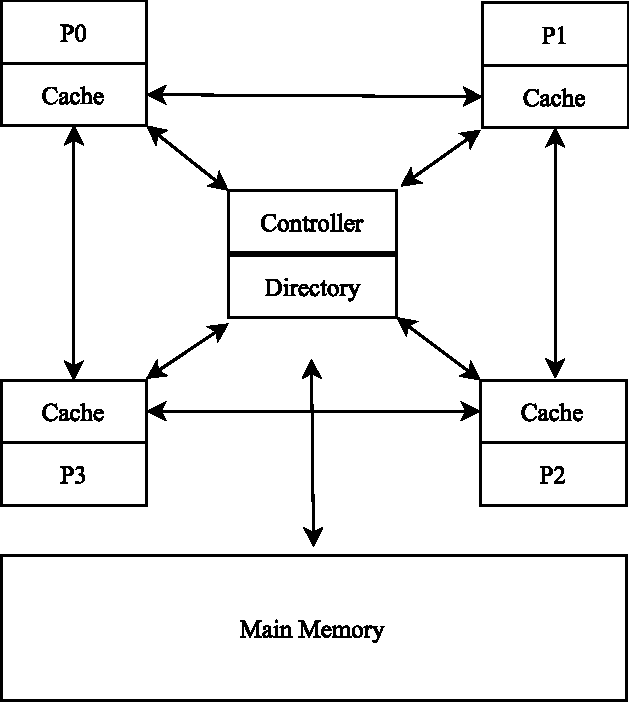
\includegraphics{figs/DirectoryCache.pdf}
\caption{Diagram of the architecture used with the directory-based protocol.}
\label{fig:dir-arch}
\end{figure}

In order to verify the correctness of the implementation, we show several small
traces executed in verbose mode.

\begin{figure}[h]
\begin{verbatim}
P2 W 10
Processor P2 writes word in address 10, with tag 0 and slot 2.
A cache miss occurred. Data transferred from main memory.
A total of 0 invalidations were required.
(18 cycles taken)
P3 R 10
Processor P3 reads word in address 10, with tag 0 and slot 2.
A cache miss occurred. Data transferred from remote processor
in Exclusive state with distance 1.
A protocol writeback was required by processor P2.
(13 cycles taken)
P1 W 10
Processor P1 writes word in address 10, with tag 0 and slot 2.
A cache miss occurred. Data transferred from remote processor
in Shared state with distance 1.
A total of 2 invalidations were required.
(13 cycles taken)
\end{verbatim}
\caption{(Directory-based Protocol) Test case: Write at P1; Local cache line in I state, Remote cache line at
P2, P3 in S state.}
\end{figure}

\begin{figure}[h]
\centering
\begin{subfigure}{0.48\textwidth}
\begin{verbatim}
Trace 1
Total Reads: 163840
Total Writes: 32768
Total Requests: 196608
Hit Rate: 0.912679036458
Direct Write: 24440
Invalidations: 0
Invalidation Sent: 0
Private Accesses: 179440
Remote Accesses: 8427
Off-chip Accesses: 8741
Protocol Writeback: 51
Replacement Writeback: 6357
Total Cycle Count: 584129
Mean Cycle Per Req.: 2.9710337321
\end{verbatim}
\end{subfigure}
\begin{subfigure}{0.48\textwidth}
\begin{verbatim}
Trace 2
Total Reads: 507093
Total Writes: 76462
Total Requests: 583555
Hit Rate: 0.995224100556
Direct Write: 74622
Invalidations: 0
Invalidation Sent: 0
Private Accesses: 580768
Remote Accesses: 2280
Off-chip Accesses: 507
Protocol Writeback: 455
Replacement Writeback: 0
Total Cycle Count: 1195843
Mean Cycle Per Req.: 2.04923786104
\end{verbatim}
\end{subfigure}
\caption{Statistics for the Directory-based protocol on Traces 1 and 2.}
\end{figure}


\section{MESI Snooping Protocol with Second-Level Shared Cache} \label{sec:mesi-snooping-2lvl}

For the optimised snooping protocol, we implemented the MESI protocol
with a second-level shared cache. In the results we show that the MESI protocol
alone can improve over the MSI snooping protocol, while the 1KB second-level
shared cache provides a very small improvement.
We consider the architecture illustrated in Figure~\ref{fig:dir-arch},
where the cores are inter-connected by an unidirectional ring.
The controller is supposed to be able to probe the shared cache in one cycle.

\begin{figure}
\centering
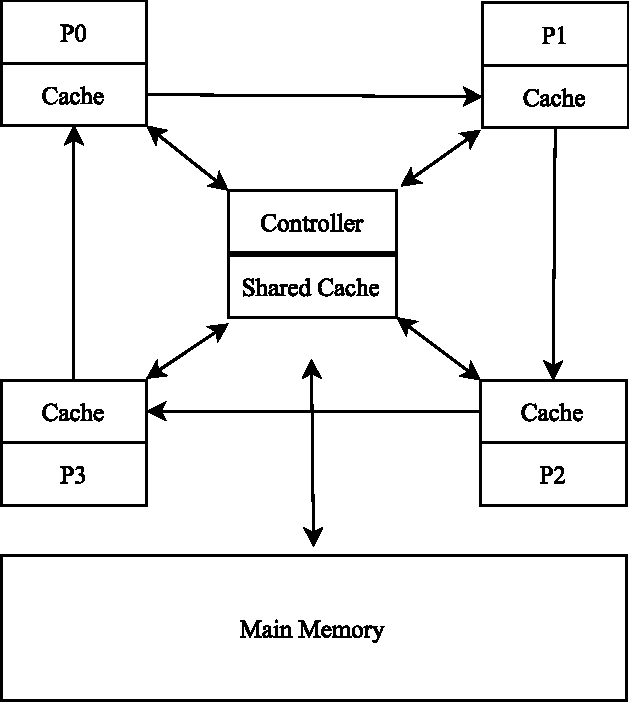
\includegraphics{figs/MESISnooping2LevelCache.pdf}
\caption{Diagram of the architecture used with the MESI snooping protocol with
the second-level shared cache close to the memory controller.}
\label{fig:mesi-arch}
\end{figure}


\begin{figure}[h]
\centering
\begin{subfigure}{0.48\textwidth}
\begin{verbatim}
Trace 1
Total Reads: 163840
Total Writes: 32768
Total Requests: 196608
Hit Rate: 0.954778035482
Direct Write: 32717
Invalidations: 51
Invalidation Sent: 153
Private Accesses: 187717
Remote Accesses: 150
Off-chip Accesses: 8741
Protocol Writeback: 51
Replacement Writeback: 6357
Total Cycle Count: 663037
Mean Cycle Per Req.: 3.37238057454
\end{verbatim}
\end{subfigure}
\begin{subfigure}{0.48\textwidth}
\begin{verbatim}
Trace 2
Total Reads: 507093
Total Writes: 76462
Total Requests: 583555
Hit Rate: 0.855568027007
Direct Write: 38839
Invalidations: 48557
Invalidation Sent: 111159
Private Accesses: 499271
Remote Accesses: 83641
Off-chip Accesses: 643
Protocol Writeback: 35757
Replacement Writeback: 0
Total Cycle Count: 2432247
Mean Cycle Per Req.: 4.16798245238
\end{verbatim}
\end{subfigure}
\caption{Statistics for the MESI Snooping protocol with 1KB of Shared Cache on Traces 1 and 2.}
\end{figure}

\section{Results}

\begin{figure}[h]
\centering
\begin{subfigure}{0.48\textwidth}
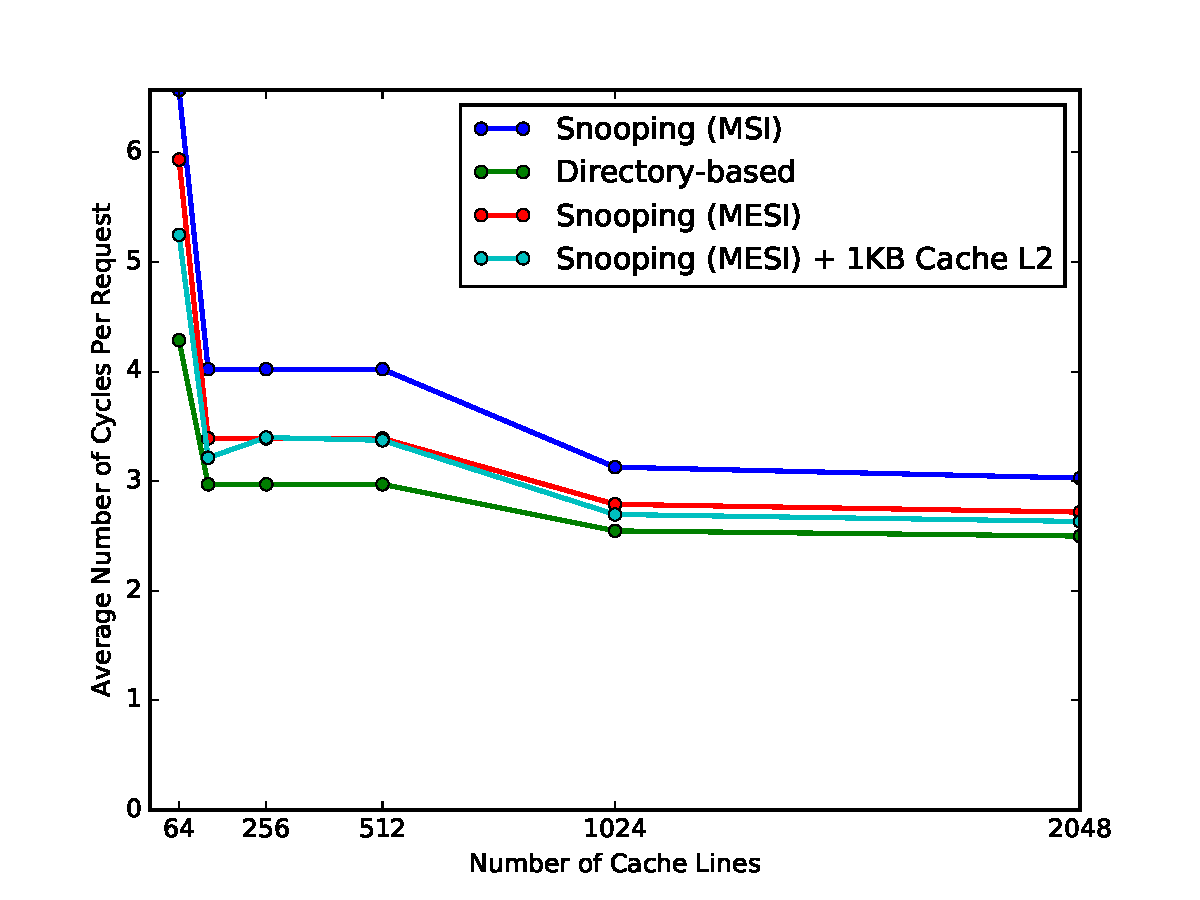
\includegraphics[width=\textwidth]{figs/fig-1-1.pdf}
\end{subfigure}
\begin{subfigure}{0.48\textwidth}
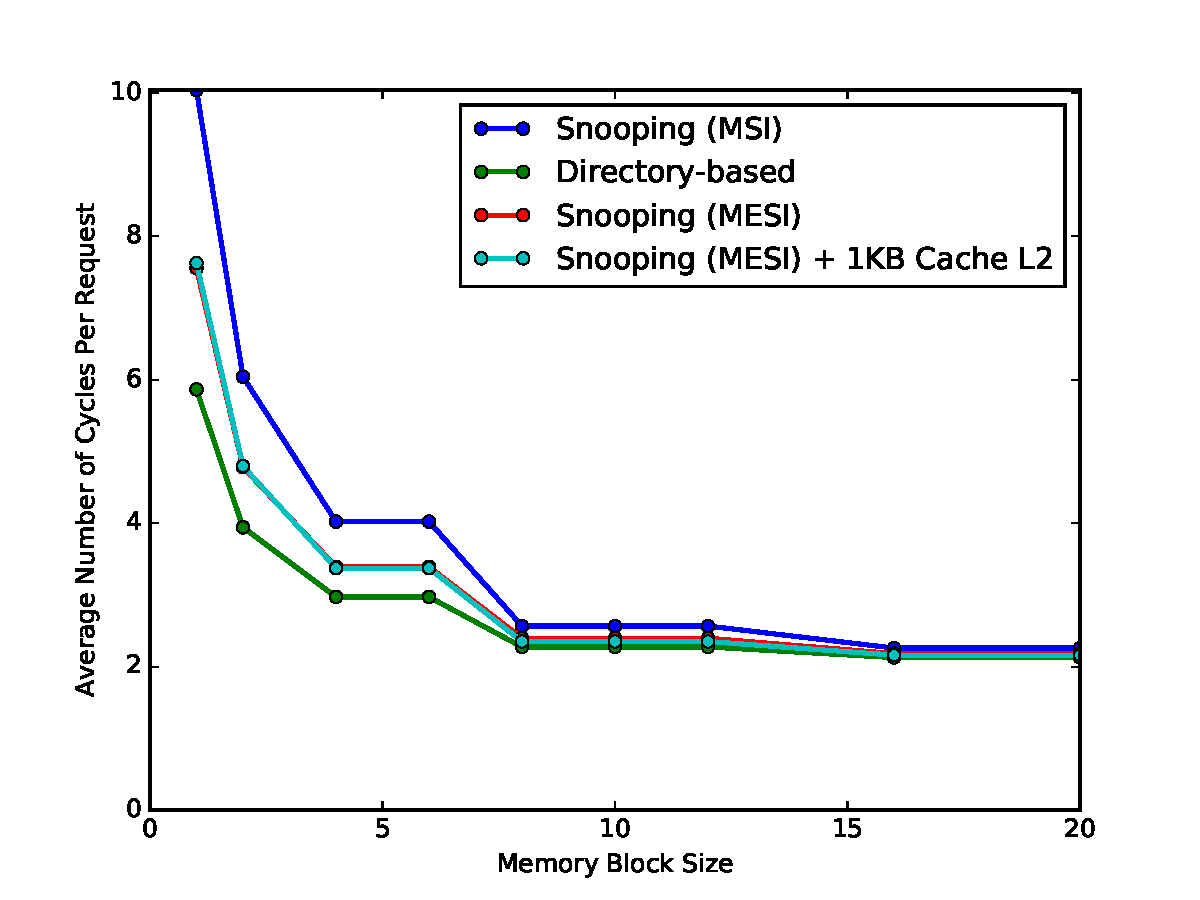
\includegraphics[width=\textwidth]{figs/fig-1-2.pdf}
\end{subfigure}
\caption{Comparison of the cache-coherence protocols on Trace 1.}
\end{figure}

\begin{figure}[h]
\centering
\begin{subfigure}{0.48\textwidth}
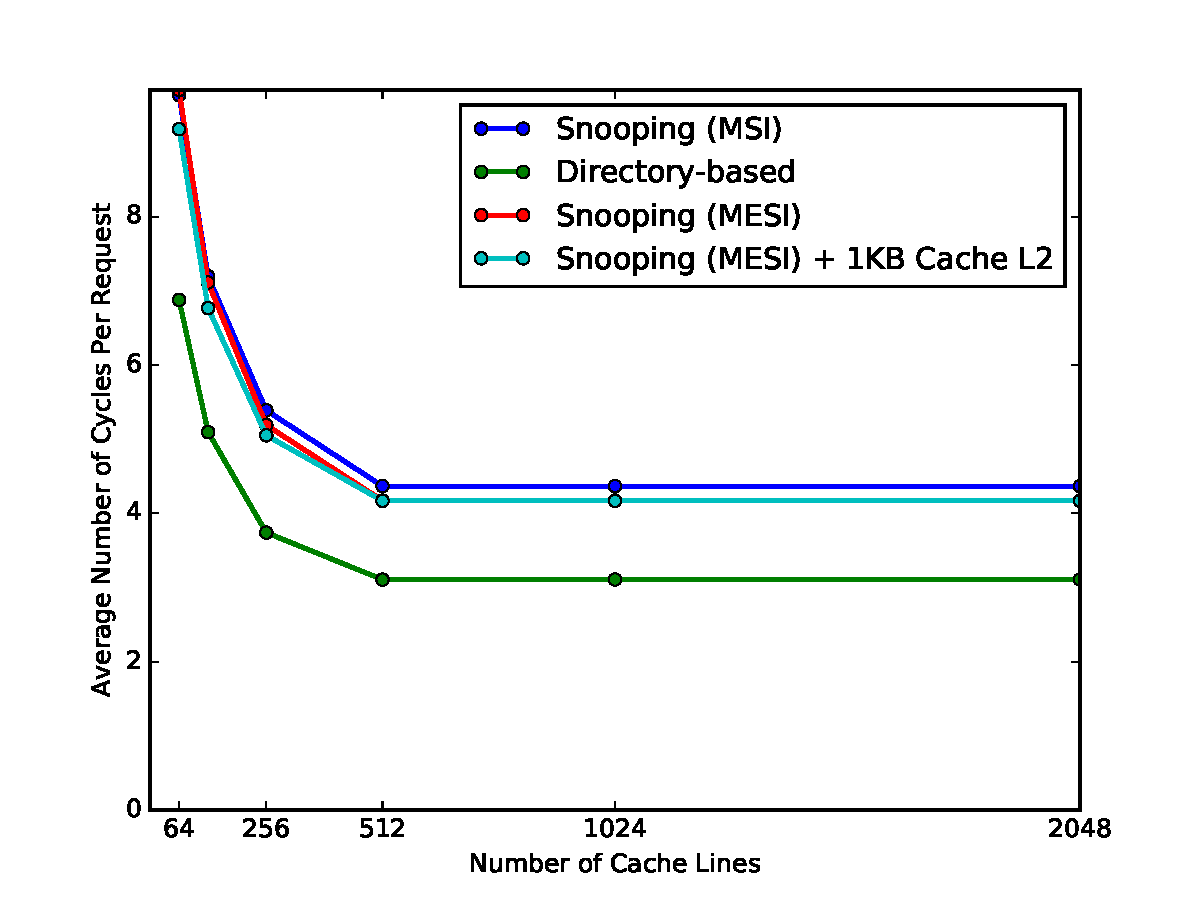
\includegraphics[width=\textwidth]{figs/fig-2-1.pdf}
\end{subfigure}
\begin{subfigure}{0.48\textwidth}
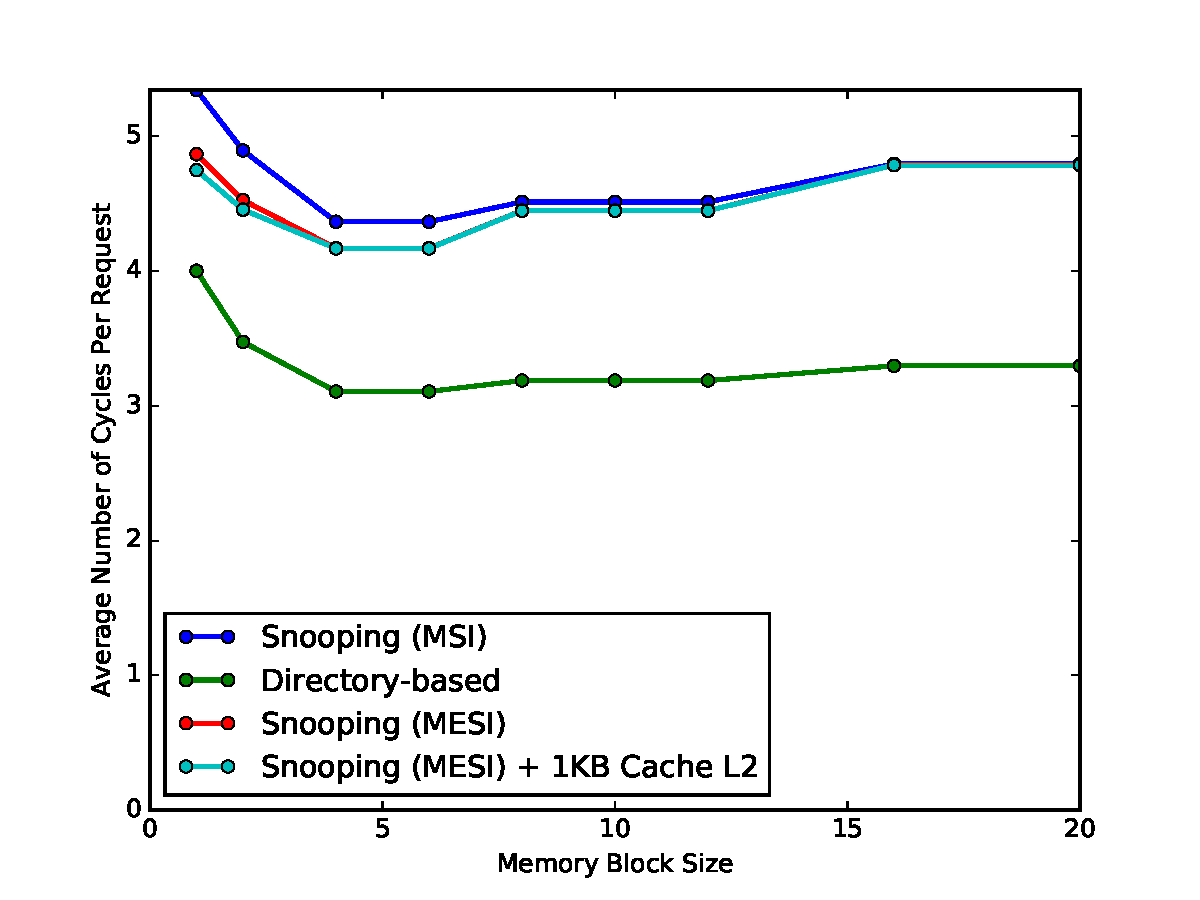
\includegraphics[width=\textwidth]{figs/fig-2-2.pdf}
\end{subfigure}
\caption{Comparison of the cache-coherence protocols on Trace 2.}
\end{figure}

\begin{figure}[h]
\centering
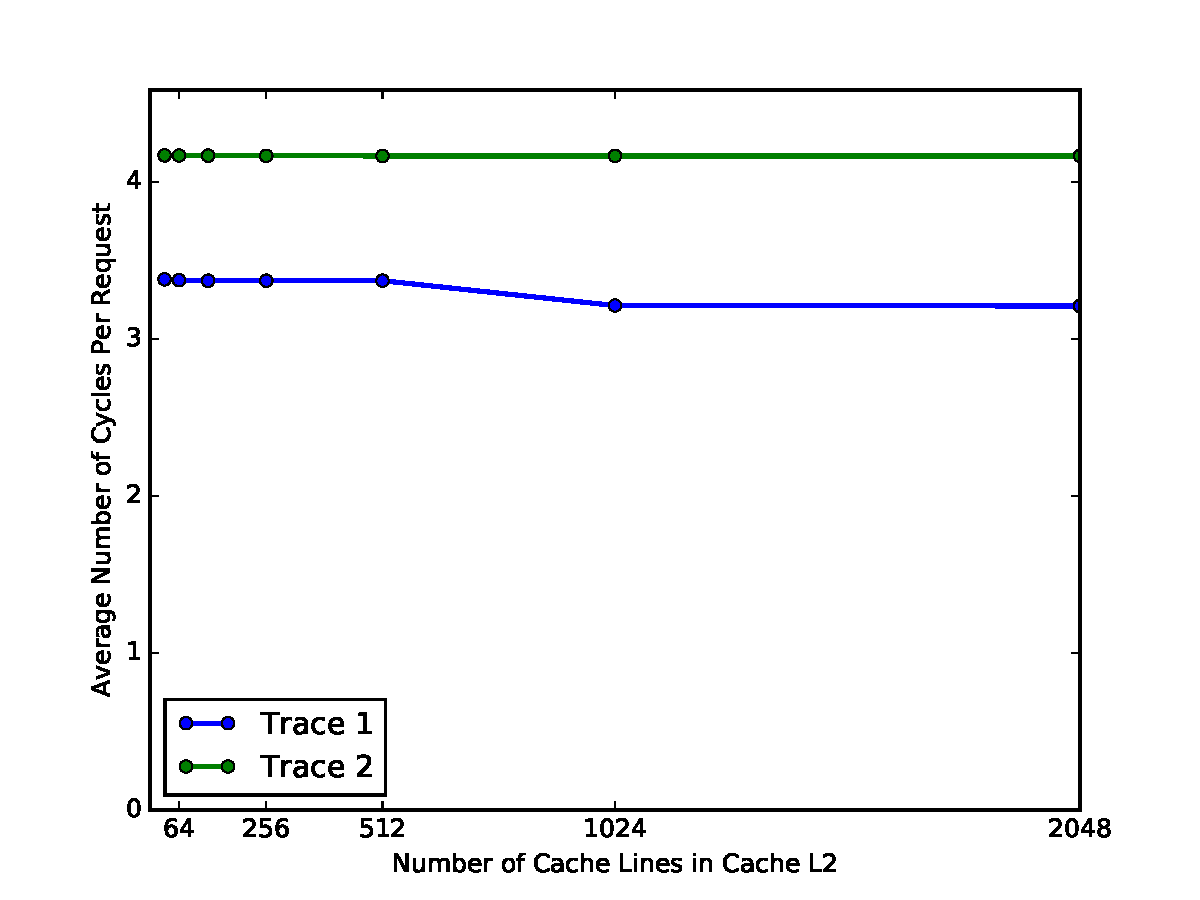
\includegraphics[width=0.6\textwidth]{figs/fig-3.pdf}
\caption{Performance of the MESI protocol with Second-Level Shared Cache, when varying the size of the shared cache.}
\end{figure}

\section{Conclusion}

From the results we can see that the directory-based protocol has the best performance amongst the protocols.
The shared cache has no major impact due to its limited size of 1KB and the simple prefetching mechanism
based on keeping the replaced blocks and prefetching a single adjacent block when reading data from the main memory.

\end{document}
